\documentclass[sn-mathphys-num,referee]{sn-jnl}
\usepackage{natbib} % For citations

%\usepackage{cite}
\usepackage{graphicx}
\usepackage{psfrag}
\usepackage{anyfontsize}
\usepackage{url}
\usepackage{color}
\usepackage{balance}
\usepackage[all]{xy}
\usepackage{xspace}
\usepackage{listings}
\usepackage{adjustbox}
\usepackage{array,booktabs,arydshln,xcolor}
\usepackage{tikz}
\usetikzlibrary{shapes,patterns,calc,shapes.geometric,arrows,positioning,backgrounds}
\usepackage{float}
\usepackage{makecell}
\usepackage{multirow}
\usepackage{xcolor}
\usepackage{url}
\usepackage{amsthm}
\usepackage{float}
\usepackage{amsmath}
\usepackage[capitalise]{cleveref}
\usepackage{soul}
\usepackage[inline]{enumitem}
\usepackage{xcolor}
\usepackage{amssymb}
\usepackage{pifont}
\usepackage{epstopdf}
\usepackage{subcaption}
\colorlet{OurColor}{blue}
\graphicspath{{Images/}}

\theoremstyle{definition}
\newtheorem{theorem}{Theorem}[section]
\newtheorem{definition}{Definition}
\newtheorem{example}{Example}[section]

% please place your own definitions here and don't use \def but
% \newcommand{}{}
\newcommand\CH[1]{\textcolor{blue}{{CHIARA - }{#1}}}
\newcommand\CL[1]{\textcolor{red}{{CLAUDIO - }{#1}}}
\newcommand\MC[1]{\textcolor{green}{{MARCO - }{#1}}}
\newcommand\AJ[1]{\textcolor{orange}{{AJ - }{#1}}}
\newcommand{\job}[1]{\ensuremath{J_{#1}}}
\newcommand{\trans}[1]{\ensuremath{T_{#1}}}
\newcommand{\coalition}[1]{\ensuremath{C_{#1}}}
\newcommand{\org}[1]{\ensuremath{o_{#1}}}
\newcommand{\Org}[1]{\ensuremath{O_{#1}}}
\newcommand{\dataset}[1]{\ensuremath{D_{#1}}}
\newcommand{\orc}[1]{\ensuremath{Orc_{#1}}}
\newcommand{\G}{\ensuremath{G}}
\newcommand{\V}{\ensuremath{V}}
\newcommand{\E}{\ensuremath{E}}
\newcommand{\vi}[1]{\ensuremath{v_{#1}}}

\begin{document}

\title[Maximizing Data Quality While Ensuring Data Protection in Service-Based Data Pipelines]{Maximizing Data Quality While Ensuring Data Protection in Service-Based Data Pipelines}
% \title[Maximizing Data Quality While Ensuring Data Protection in Service-Based Data Pipelines]{Maximizing Data Quality While Ensuring Data Protection in Service-Based Data Pipelines}
% \title[Service-Based Data Pipelines: Maximizing Data Quality While Ensuring Data Protection Requirements]{Service-Based Data Pipelines: Maximizing Data Quality While Ensuring Data Protection Requirements}
% \title[Service-Based Data Pipelines: Maximizing Data Quality While Ensuring Data Protection]{Service-Based Data Pipelines: Maximizing Data Quality While Ensuring Data Protection}
\keywords{Access Control, Big Data, Data Pipelines, Data Protection, Data Quality, Privacy}
%Data Transformation, Data Ingestion}

\author[1]{\fnm{Antongiacomo} \sur{Polimeno}}\email{antongiacomo.polimeno@unimi.it}
\author[1]{\fnm{Chiara} \sur{Braghin}}\email{chiara.braghin@unimi.it}
\author[1]{\fnm{Marco} \sur{Anisetti}}\email{marco.anisetti@unimi.it}
\author*[1]{\fnm{Claudio A.} \sur{Ardagna}}\email{claudio.ardagna@unimi.it}

\affil[1]{\orgdiv{Dipartimento di Informatica}, \orgname{Università degli Studi di Milano}, \orgaddress{\city{Milano}, \country{Italy}}}

\maketitle

\begin{abstract}
~Today, the increasing ability of collecting and managing huge volume of data, coupled with a paradigm shift in service delivery models, has significantly enhanced scalability and efficiency in data analytics, particularly in multi-tenant environments. Data are today treated as digital products, which are managed and analyzed by multiple services orchestrated in data pipelines. {\color{OurColor}This paradigm shift towards distributed systems built as service-based data pipelines does not find any counterparts in the definition of new data governance techniques that properly manage data across the pipeline lifecycle, calling for innovative solutions to data pipeline management that primarily seek to balance data quality and data protection. Departing from the state of the art that traditionally targets single services and systems, and optimizes data protection and data quality as independent factors}, we propose a framework that enhances service selection and composition in service-based data pipelines to the aim of maximizing data quality, while providing a minimum level of data protection. Our approach first retrieves a set of candidate services compatible with data protection requirements in the form of access control policies; it then selects the subset of compatible services, to be integrated within the data pipeline, which maximizes the overall data quality. Being our approach NP-hard, a sliding-window heuristic is defined and experimentally evaluated in terms of performance and quality with respect to the exhaustive approach. Our results demonstrate a significant reduction in computational overhead, while maintaining high data quality.
\end{abstract}

\tikzset{
  do path picture/.style={%
      path picture={%
          \pgfpointdiff{\pgfpointanchor{path picture bounding box}{south west}}%
          {\pgfpointanchor{path picture bounding box}{north east}}%
          \pgfgetlastxy\x\y%
          \tikzset{x=\x/2,y=\y/2}%
          #1
        }
    },
  cross/.style={do path picture={
          \draw [line cap=round ] (-1,-1) -- (1,1) (-1,1) -- (1,-1);
        }},
  plus/.style={do path picture={
          \draw [line cap=round] (-3/4,0) -- (3/4,0) (0,-3/4) -- (0,3/4);
        }}
}

\section{Introduction}
The usage of multitenancy coupled with cloud infrastructure represents a paradigm shift in the big data scenario, redefining scalability and efficiency in data analytics. Multitenancy enables multiple users to share resources, such as computing power and storage, optimizing resource utilization and reducing operational costs. Leveraging cloud infrastructure further enhances flexibility and scalability.
%allowing organizations to dynamically allocate resources based on demand while ensuring seamless access to cutting-edge data analytics tools and services.
%
The flip side of multitenancy is the increased complexity of data governace: the shared model introduces unique security challenges, as tenants may have different security requirements, levels of access, and data sensitivity. Adequate measures such as encryption, access control mechanisms, and data anonymization techniques must be implemented to safeguard data against unauthorized access and ensure compliance with regulatory requirements such as GDPR or HIPAA.
%
As a consequence, achieving a balance between data protection and data quality is crucial, as the removal or alteration of personally identifiable information from datasets to safeguard individuals' privacy can compromise the accuracy of analytics results.

So far, all research endeavors have been concentrated on exploring these two issues separately: on one hand, the concept of data quality, encompassing accuracy, reliability, and suitability, has been investigated to understand the implications in analytical contexts. Although extensively studied, these investigations often prioritize enhancing the quality of source data rather than ensuring data quality throughout the entire processing pipeline, or the integrity of outcomes derived from data. On the other hand, there is a focus on data privacy and security, entailing the protection of confidential information and adherence to rigorous privacy regulations.

A valid solution requires a holistic approach that integrates technological solutions, organizational policies, and ongoing monitoring and adaptation to emerging threats and regulatory changes. The implementation of robust access control mechanisms, ensuring that only authorized users can access specific datasets or analytical tools is just an essential initial step.
Indeed, we identified some additional requirements. First, data protection requirements should be identified at each stage of the data lifecycle, potentially incorporating techniques like data masking and anonymization to safeguard sensitive information, thereby preserving data privacy while enabling sharing and analysis. Second, data lineage should be prioritized, fostering a comprehensive understanding and optimization of data flows and transformations within complex analytical ecosystems. 

When evaluating a solution meeting these criteria, the following questions naturally arise:
\begin{enumerate}
\item How does a robust data protection policy affect analytics?
%What impact does a robust and strong data protection policy have on analytics?
%How does a strong data protection policy influence analytics?
\item When considering a pipeline, is it more advantageous to perform data protection transformations at each step rather than filtering all data at the outset? 
\item In a scenario where a user has the option to choose among various candidate services, how might these choices affect the analytics?
\end{enumerate}
%
Based on the aforementioned considerations, we propose a data governance framework customized for modern data-driven pipelines, designed to mitigate privacy and security risks. The primary objective of this framework is to facilitate the assembly of data processing services, with a central focus on the selection of those services that optimize data quality, while upholding privacy and security requirements. 

In our solution, each element in the pipeline is tagged with \textit{annotations} to specify data protection requirements expressing transformation on data to enforce data protection, as well as functional specifications on services expressing data manipulations carried out during services execution. For each element in the pipeline, there is a catalog of candidate services among which the user running it can choose. Services may be functionally equivalent (i.e., they perform the same tasks), but have different security policies, more or less restrictive depending on the organization or service provider they belong to.
Our data governance approach is based on the belief that maintaining a larger volume of data leads to higher data quality, thus our service selection approach focuses on maximizing data quality by retaining the maximum amount of information when applying data protection transformations. 
We have a running example on which we conducted experiments to provide an initial answer to the questions highlighted earlier.

The primary contributions of the paper can be summarized as follows:
\begin{enumerate}
  \item Enriching services with meta-data that describes both data protection and functional requirements;
  \item Proposing a parametric heuristic tailored to address the computational complexity of the NP-hard service selection problem;
  \item Evaluating the performance and quality of the algorithm through experiments conducted using the dataset from the running example.
\end{enumerate}
%
The remainder of the paper is structured as follows: Section 2, presents our system model, illustrating a reference scenario where data is owned by multiple organizations. In Section \ref{sec:template}, we introduce the pipeline template and describe the annotations. In Section \ref{sec:instance}, we describe the process of template instantiaton. In Section \ref{sec:heuristics}, we introduce the quality metrics used by the selection algorithm and the heuristic solving the service selection problem. Section \ref{sec:experiment} outlines the experiments conducted. Section \ref{sec:related} discusses the existing solutions. Section \ref{sec:conclusions} concludes the paper.
\section{Requirements and System Model}\label{sec:requirements}
Big data is highly dependent on cloud-edge computing, which makes extensive use of multitenancy.
Multitenancy permits sharing one instance of infrastructures, platforms or applications by multiple tenants to optimize costs.
This leads to common scenarios where a service provider offers subscription-based analytics capabilities in the cloud,
or a single data lake is accessed by multiple customers.
Thus, it is a common situation to have a big data pipeline where data and services belong to various organizations,
posing a serious risk of potential privacy and security violation.
In the following of this section,
we present our system model (Section \ref{sec:systemmodel}),
the requirements driving our work (Section \ref{sec:accesscontrol_req}),
and our reference scenario (Section \ref{sec:reference}).
\AG{
  In our context a \user, aims to implement a data pipeline to facilitate analysis or transformation procedures on some data.
  Policies governing the data are established, which can originate from the \user, third-party entities, or regulatory frameworks.
  For instance, a policy may restrict the execution of processing operations to a specific geographic region.
  The \user is provided with a set of pipeline templates. Each template represents a blank pipeline with the necessary steps but without the specific services.
  To instantiate the template, the user is given the opportunity to choose, for each step of the pipeline, from a collection of candidate services that are functionally equivalent and comply with the specified policies.
  These services are subsequently ranked based on their ability to retain the maximum amount of data while maintaining an equivalent level of privacy.
  Underlying our investigation is the assumption that a greater quantity of preserved data corresponds to enhanced data quality.
}
\subsection{System Model}\label{sec:systemmodel}

\begin{itemize}
  \item User owns some data and wants to perform some analytics on it
  \item Choose a pipeline template and a wanted level of privacy
  \item The template has lambda, signed
  \item Policy is a set of rules
  \item Match the policy with the lambda
  \item Compares services that match the policy ranking them based on quality
  \item Choose the best service
  \item The composite service is executed
\end{itemize}

\AG{Our system model aims to achieve an optimal service composition to ensure privacy and data quality.
  Within this context, we contemplate an interconnected sequence of services, establishing a pipeline where individual nodes signify distinct services.
  Each stage within the pipeline undertakes the task of data transformation or processing, with the resulting output serving as the input for the subsequent service.
  This model encapsulates what we refer to as a template, visually presented in Figure \ref{fig:service_composition_template}.
  In order to instantiate the template, the selection of services to be executed at each step of the pipeline becomes imperative.
  At each step, there exists a collection of functionally equivalent services that differ in terms of annotation and data transformation.
  These services are annotated with a set of requirements that encompass crucial details, including the owner's information, as well as other pertinent metadata such as the region of execution, for example.
  The annotations play a pivotal role in the creation of policies that determine the eligibility of a service for deployment.
  By enforcing such policies, the set of candidate services for a given step is reduced.
  The remaining services undergo evaluation based on their potential impact on the data transformation process.
  Preference is given to the service that maximizes data quality while ensuring an equal level of data privacy.
  This evaluation process aids in identifying the most suitable service for a particular step in the pipeline.
  Upon the selection of the most appropriate service for each step, the instantiation of the pipeline is deemed complete.
  Consequently, the pipeline becomes ready for execution, with the assurance that the chosen services align with the specified requirements and optimize the desired outcomes.
}

% We formally model a Big Data analytics pipeline as follows.

% \begin{definition}[Big Data Analytics Pipeline] \label{def:pipeline}
%   A Big Data Analytics pipeline \G(\V,\E) is a direct acyclic graph having a root \vi{r}$\in$\V, a vertex \vi{i}$\in$\V$_I$$\subseteq$\V\ for each job \job{i} invocation, two additional vertices \vi{c},\vi{m}$\in$\V$_{\otimes}$$\subset$\V\ for each alternative ($\otimes$) structure modeling the alternative execution (\emph{choice}) of operations and the retrieval (\emph{merge}) of the results,
%     respectively, and two additional vertices \vi{f},\vi{j}$\in$\V$_{\oplus}$$\subset$\V\ for each parallel ($\oplus$) structure modeling the contemporary execution (\emph{fork}) of operations and the integration (\emph{join}) of their results, respectively.
% \end{definition}

% We note that each vertex \vi{i} model a job \job{i} provided by an organization \org{i}.
% We also note that an analytics pipeline can be deployed following a centralized or a decentralized approach as discussed in detail in Section \ref{sec:architecture}.

\begin{figure}[!t]
  \includegraphics[width=0.98\columnwidth]{generaleFig1.pdf}
  \caption{Big Data Analytics pipeline graphs with a coalition of organization for a given processing lineage.}\label{fig:BDpipeline}
\end{figure}

Figure~\ref{fig:BDpipeline} shows an overview of our system model.

%Solid arrows present the typical batch or analytics model generation flows. Dashed arrows present typical streaming or prediction flows. \CH{togliere dalla figura la linea che separa le due procedure e le scritte ingestion procedure e analytics procedure?}
%The coalition creation is driven by missions including emergency and disaster management, humanitarian operations, or simply interdependent organizations.
%\CH{Qui ho introdotto solo il termine coalition, va spiegato anche il termine federation?}


\section{Policy}

\subsection{Annotations}
\subsection{Transformation}
\subsection{Policy}

\subsubsection{Policy Decision/Policy Matching}
\subsubsection{Policy Enforcement}
\subsubsection{Policy Evaluation}
\section{Pipeline Template}\label{sec:template}
Our approach integrates data protection and data management into the service pipeline using annotations. To this aim, we extend the service pipeline in \cref{def:pipeline} with: \emph{i)} data protection annotations that express transformations on data, ensuring compliance with data protection requirements, \emph{ii)} functional annotations that express data manipulations carried out during service execution.
These annotations enable the implementation of an advanced data lineage, tracking the entire data lifecycle by monitoring changes that result from functional service execution and data protection requirements.

In the following, we first introduce the annotated service pipeline, called pipeline template (Section \ref{sec:templatedefinition}). We then present both functional annotations (Section \ref{sec:funcannotation}) and data protection annotations (Section \ref{sec:nonfuncannotation}), providing an example of a pipeline template in the context of the reference scenario.

\subsection{Pipeline Template Definition}\label{sec:templatedefinition}
Given the service pipeline in Definition~\ref{def:pipeline}, we use annotations to express data protection requirements to be enforced on data and functional requirements on the services to be integrated in the pipeline. Each service vertex in the service pipeline is labeled with two mapping functions forming a pipeline template:
\begin{enumerate*}[label=\textit{\roman*})]
  \item an annotation function \myLambda:$\V_S\rightarrow$\P{} that associates a set of data protection requirements, in the form of policies $p$$\in$\P{}, with each vertex \vi{i}$\in$$\V_S$;
  \item an annotation function \myGamma:$\V_S\rightarrow$\F{} that associates a functional service description $F_i\in\F{}$ with each vertex \vi{i}$\in$$\V_S$.
\end{enumerate*}

The template is formally defined as follows.

\vspace{0.5em}

\begin{definition}[Pipeline Template] \label{def:template}
  Given a service pipeline G(\V,\E), a pipeline template \tChartFunction is a direct acyclic graph extended with two annotation functions:
  \begin{enumerate}%[label=\textit{\roman*}]
    \item \emph{Data Protection Annotation} \myLambda that assigns a label \myLambda(\vi{i}) to each vertex $\vi{i}\in\V_S$. Label \myLambda(\vi{i}) corresponds to a set \P{i} of policies $p_j$ to be satisfied by service $s_i$ represented by \vi{i};
    \item \emph{Functional Annotation} \myGamma that assigns a label \myGamma(\vi{i}) to each vertex $\vi{i}\in\V_S$. Label \myGamma(\vi{i}) corresponds to the functional description $F_i$ of service $s_i$ represented by \vi{i}.
  \end{enumerate}
\end{definition}

\vspace{0.5em}

We note that, at this stage, the template is not yet linked to any service. We also note that policies $p_j$$\in$\P{i} in \myLambda(\vi{i}) are combined using logical OR, meaning that the access decision is positive if at least one policy $p_j$ evaluates to \emph{true}. The pipeline template of the service pipeline of \cref{fig:reference_scenario} is depicted in \cref{fig:service_composition_template}.

      \begin{figure}[ht!]
        \centering
        \newcommand{\function}[1]{$\ensuremath{\myLambda_{#1},\myGamma_{#1}}$}
        \begin{tikzpicture}[scale=0.9]
          % vertexes
          \node[draw, circle, fill,text=white,minimum size=1 ] (sr) at (0,0) {};
          \node[draw, circle, plus,minimum size=1.5em] (plus) at (1.5,0) {};
          \node[draw, circle] (s1) at (3,1.7) {$\vi{3}$};
          \node[draw, circle] (s2) at (3,-1.7) {$\vi{1}$};
          \node[draw, circle] (s3) at (3,0) {$\vi{2}$};


          \node[draw, circle] (s4) at (4.5,0) {$\vi{4}$};

          \node[draw, circle] (s5) at (6,0) {$\vi{5}$};

          \node[draw, circle] (s7) at (7.5,0) {$\vi{6}$};
          \node[draw, circle] (s8) at (9,0) {$\vi{7}$};
          % Text on top
          \node[above] at (sr.north)  {$\vi{r}$};

          \node[above] at (s1.north)  {\function{3}};

          \node[above] at (s2.north)  {\function{1}};
          \node[above] at (s3.north)  {\function{2}};
          \node[above] at (s4.north)  {\function{4}};
          \node[above] at (s5.north)  {\function{5}};
          \node[above] at (s7.north)  {\function{6}};
          \node[above] at (s8.north)  {\function{7}};
          % Connection

          \draw[->] (sr) -- (plus);
          \draw[->] (plus) -- (s1);
          \draw[->] (plus) -- (s2);
          \draw[->] (plus) -- (s3);

          \draw[->] (s1) -- (s4);
          \draw[->] (s2) -- (s4);
          \draw[->] (s3) -- (s4);
          \draw[->] (s4) -- (s5);
          \draw[->] (s5) -- (s7);
          \draw[->] (s7) -- (s8);

        \end{tikzpicture}
        \caption{Pipeline Template}
        \label{fig:service_composition_template}
      \end{figure}

      \subsection{Data Protection Annotation}\label{sec:nonfuncannotation}
      Data Protection Annotation \myLambda\ expresses data protection requirements in the form of access control policies. We consider an attribute-based access control model that offers flexible fine-grained authorization and adapts its standard key components to address the unique characteristics of a big data environment. Access requirements are expressed in the form of policy conditions that are defined as follows.

      \vspace{0.5em}

      \begin{definition}[Policy Condition]\label{def:policy_cond}
        A \emph{Policy Condition pc} is a Boolean expression of the form $($\emph{attr\_name} op \emph{attr\_value}$)$, with op$\in$\{$<$,$>$,$=$,$\neq$,$\leq$,$\geq$\}, \emph{attr\_name} an attribute label, and \emph{attr\_value} the corresponding attribute value.
      \end{definition}

      \vspace{0.5em}

      Built on policy conditions, an access control policy is then defined as follows.
      \vspace{0.5em}
      \begin{definition}[Policy]\label{def:policy_rule}
        A {\it policy p}$\in$\P{} is 5-uple $<$\textit{subj}, \textit{obj}, \textit{act}, \textit{env}, \textit{\TP}$>$ that specifies who (\emph{subject}) can access what (\emph{object}) with action (\emph{action}), in a specific context (\emph{environment}) and under specific obligations (\emph{data transformation}).
      \end{definition}

      \vspace{0.5em}

      More in detail, \textit{subject subj} specifies a service $s_i$ issuing an access request to perform an action on an object. It is a set \{$pc_i$\} of \emph{Policy Conditions} as defined in Definition \ref{def:policy_cond}. For instance, (classifier$=$``SVM'') specifies a service providing a SVM classifier. We note that \textit{subj} can also specify conditions on the service owner (\textit{e.g.}, owner\_location$=$``EU'') and the service user (\textit{e.g.}, service\_user\_role$=$``DOC Director'').

      \textit{Object obj} defines the data governed by the access policy. In this case, it is a set \{$pc_i$\} of \emph{Policy Conditions} on the object's attributes. 
      For instance, \{(type$=$``dataset''), (region$=$``CT'')\} refers to an object of type dataset and whose region is Connecticut.

      \textit{Action act} specifies the operations that can be performed within a big data environment, from traditional atomic operations on databases (e.g., CRUD operations) to coarser operations, such as an Apache Spark Direct Acyclic Graph (DAG), Hadoop MapReduce, an analytics function call, and an analytics pipeline.

      \textit{Environment env} defines a set of conditions on contextual attributes, such as time of the day, location, IP address, risk level, weather condition, holiday/workday, and emergency. It is a set \{$pc_i$\} of \emph{Policy Conditions} as defined in Definition \ref{def:policy_cond}. For instance, (time$=$``night") refers to a policy that is applicable only at night.

      \textit{Data Transformation \TP} defines a set of security and privacy-aware transformations on \textit{obj} that must be enforced before any access to data is given. Transformations focus on data protection, as well as on compliance to regulations and standards, in addition to simple format conversions. For instance, let us define three transformations that can be applied to the dataset in \cref{tab:dataset}, each performing different levels of anonymization:
      \begin{enumerate*}[label=\roman*)]
        \item level \emph{l0} (\tp{0}): no anonymization;
        \item level \emph{l1} (\tp{1}): partial anonymization with only first and last name being anonymized;
        \item level \emph{l2} (\tp{2}): full anonymization with first name, last name, identifier and age being anonymized.
      \end{enumerate*}

Access control policies $p_j$$\in$\P{i} annotating a vertex \vi{i} in a pipeline template $G^{\myLambda,\myGamma}$ specify the data protection requirements that a candidate service must fulfill to be selected in the pipeline instance. Section~\ref{sec:instance} describes the selection process and the pipeline instance generation.

\subsection{Functional Annotations}\label{sec:funcannotation}
A proper data management approach must track functional data manipulations across the entire pipeline execution, defining the functional requirements of each service operating on data.
To this aim, each vertex \vi{i}$\in\V_S$ is annotated with a label \myGamma(\vi{i}), corresponding to the functional description $F_i$ of the service $s_i$ represented by \vi{i}.
$F_i$ describes the functional requirements, such as API, inputs, expected outputs.
It also specifies a set \TF{} of data transformation functions \tf{i}, which can be triggered during the execution of the corresponding service $s_i$.

Function $\tf{i}$$\in$$\TF{}$ can be:
\begin{enumerate*}[label=\textit{\roman*})]
  \item an empty function \tf{\epsilon} that applies no transformation or processing on the data;
  \item an additive function \tf{a} that expands the amount of data received, for example, by integrating data from other sources;
  \item a transformation function \tf{t} that transforms some records in the dataset without altering the domain;
  \item a transformation function \tf{d} (out of the scope of this work) that changes the domain of the data by applying, for instance, the PCA.
\end{enumerate*}

For simplicity but with no loss of generality, we assume that all candidate services meet functional annotation \F{} and that \TF{}=\tf{}. As a consequence, all candidate services apply the same transformation to the data during the pipeline execution.
\subsection{Example}\label{sec:example}
\newcommand{\pone}{$\langle service,owner=dataset.owner\rangle$}
\newcommand{\ptwo}{$\langle service,owner=partner(dataset.owner) \rangle$}
\newcommand{\pthree}{$\langle service, owner \neq dataset.owner AND owner \neq partner(dataset.owner)$}


We present an example of pipeline template focusing on policy annotations. The pipeline template consists of five stages, and each stage is annotated with a policy presented in \cref{tab:anonymization}. \hl{Connecticut Prison (CTP) is the service user executing the pipeline. New York Prison and New Hampshire Prison are two partner DOC.}\hl{SPOSTARE NEL SYSTEM MODEL? SI, MA DATA OWNER DIPENDE DAL DATASET, HO MESSO SERVICE USER} We recall that \cref{tab:dataset} shows a sample of our reference dataset.

In the following we will make reference to three different type of anonymization:\hl{E' GIUSTO USARE \tf{i}? SPOSTIAMO PRIMA?}
\begin{enumerate*}[label=\roman*)]
  \item \emph{level0} (\tf{0}): no anonymization is performed;
  \item \emph{level1} (\tf{1}): the data is partially anonymized, only the first name and last name are anonymized;
  \item \emph{level2} (\tf{2}): the data is fully anonymized: first name, last name, identifier and age are anonymized.
\end{enumerate*}

Let us consider the pipeline template \tChartFunction in \cref{sec:example},
% 1° NODO %
The first stage consists of three parallel vertices (\vi{1}, \vi{2}, \vi{3}) and focuses on data collection without applying any policies.\hl{IN REALTA' APPLICHIAMO UNA POLITICA DI ACCESSO CON EMPTY TRANSFORMATION.} The functional requirement necessitates a URI as input, and the output is the downloaded dataset.

The second stage incorporates a sole vertex, which merges the three datasets obtained from the previous stages and is associated with three policies (\p{1},\p{2},\p{3}).
The policies are evaluated during the node execution:
%if the service profile matches with the data owner ($owner = ``CTP"$), \p{1} is satisfied and the data is not anonymized (\tf{1});
%if the service profile matches with a partner of the owner ($owner = ``CTP"$), \p{2} is satisfied and the data is partially anonymized (\tf{2});
%if the service profile doesn't match with a partner nor with the owner ($owner = ``CTP"$), \p{3} is satisfied and the data is fully anonymized (\tf{3}).
% 2° NODO %
%he second vertex is responsible for enriching the data.
%The service downloads the dataset from partner facilities and enhances the dataset of the Connecticut facility.
if the service is by the data owner (\pone), which means that if the service owner is the same as the dataset owner, the dataset is not anonymized (\tf{0}).
if the service is a partner of the data owner (\ptwo), which means that if the service owner is a partner of the dataset owner, the dataset is anonymized level1 (\tf{1}).
if the service is a third party (\pthree), which means that if the service owner is neither the dataset owner nor a partner of the dataset owner, the dataset is anonymized level2 (\tf{2}).
The functional requirement specifies $n$ datasets as input, and the output is the merged dataset.
% 3° NODO %
The third stage, is responsible both for data analysis/statistics and machine learning tasks.
The stage is composed of two alternative vertices respectively \vi{4}, \vi{5}.

Data analytics vertex adopts policies analogous to the second stage. The logic remains consistent:
if the service profile matches with the data owner (\pone), \p{1} is satisfied and the data computation is made on clean data (\tf{0});
if the service profile matches with a partner of the owner (\ptwo), \p{2} is satisfied and the data computation is made on data anonymized level1 (\tf{1});
if the service profile doesn't match with a partner nor with the owner (\pthree), \p{3} is satisfied and the data computation is made on data anonymized level2  (\tf{2}).
The functional requirement specifies a dataset as input, and the output is the computed statistics.
% 4° NODO %
Machine Learning vertex adopts always a level2 anonymization (\p(4)) to prevent personal identifiers from entering into the machine learning algorithm/model (\tf{2}).
The functional requirement specifies a dataset as input, and the output is the trained model or an inference.
% 5° NODO %
The fifth stage manages data storage.
If the service is within the facility itself ($\langle service,region=FACILITY"\rangle$), \p{5} is satisfied, resulting in data anonymization level1 (\tf{1}).
Otherwise, if the service is in a partner region ($\langle service,region={CT,NY,NH}"\rangle$), the data undergo anonymization level2 (\tf{2}).
The functional requirement specifies some\hl{?} data as input, and the output is the URI of the stored data.
% 6° NODO %
The sixth stage is responsible for data visualization.
As stated in policy annotation \p{6}, if the user is member of the facility itself, the data are anonymized level0 (\tf{0}).
If the user is member of a partner facility, the data are anonymized level1 (\tf{2}).
If the user is not member of the facility nor a partner, the data are anonymized level2 (\tf{3}).
The functional requirement specifies a dataset as input, and the output is the visualization of the data.

%In summary, this section has delineated a comprehensive pipeline template. This illustrative pipeline serves as a blueprint, highlighting the role of policy implementation in safeguarding data protection across diverse operational stages.
\begin{table*}[ht!]
  \centering
  \caption{Anonymization policies}
  \label{tab:anonymization}
  \bgroup
  \def\arraystretch{1.5}

  \begin{tabular}[t]{c|c|l}
    \textbf{Vertex} & \textbf{Policy} & \policy{subject}{object}{action}{environment}{transformation}                                   \\ \hline

    \vi{M}          & $\p{1}$         & \policy{\pone}{dataset}{READ}{ANY}{\tf{1}}\\
    \vi{M}          & $\p{2}$         & \policy{\ptwo}{dataset}{READ}{ANY}{\tf{2}}\\
    \vi{M}          & $\p{3}$         & \policy{\pthree}{dataset}{READ}{ANY}{\tf{3}}\\
    \vi{4}          & $\p{4}$         & \policy{ANY}{dataset}{READ}{ANY}{\tf{3}}\\
    \vi{5}          & $\p{5}$         & \policy{$\langle service\_region=``FACILITY"\rangle$}{dataset}{WRITE}{ANY}{\tf{1}}\\
    \vi{5}          & $\p{6}$         & \policy{$\langle service\_region=``\{CT,NY,NH\}"\rangle$}{dataset}{WRITE}{ANY}{\tf{2}}\\
    \vi{6}          & $\p{7}$         & \policy{$\langle user\_role=``Connecticut Prison Officer"\rangle$}{dataset} {READ}{ANY}{\tf{1}}\\
    \vi{6}          & $\p{7}$         & \policy{$\langle user\_role=``Partner Prison Officer"\rangle$}{dataset} {READ}{ANY}{\tf{2}}\\
    \vi{6}          & $\p{8}$         & \policy{$\langle user\_role=``Any"\rangle$}{dataset} {READ}{ANY}{    \tf{3}}\\
  \end{tabular}
  \begin{tabular}[t]{c|c|c}
    \textbf{\tf{i}} & \textbf{Level} & \textbf{Columns Anonymized}                  \\\hline
    \tf{0}          & Level0         & $anon(\varnothing)$                        \\
    \tf{1}          & level1         & $anon(FIRST\_NAME, LAST\_NAME)$                \\
    \tf{2}          & level2         & $anon(FIRST\_NAME, LAST\_NAME, IDENTIFIER, AGE)$ \\
  \end{tabular}
  %   % \begin{tabular}[t]{ccc}
  %   %   \toprule
  %   %   \textbf{Stage} & \textbf{Policy} & \textbf{Service} \\
  %   %   \midrule
  %   %   \vi{1}         & $p_1$           & $s_1$            \\
  %   %   \vi{1}         & $p_1$           & $s_2$            \\
  %   %   \vi{2}         & $p_2$           & $s_3$            \\
  %   %   \vi{2}         & $p_2$           & $s_4$            \\
  %   %   \vi{3}         & $p_3$           & $s_5$            \\
  %   %   \vi{3}         & $p_3$           & $s_6$            \\
  %   %   \bottomrule
  %   % \end{tabular}
  %   % \hspace{1em}
  %   \egroup
\end{table*}

\vspace{2em}

\begin{figure}[ht!]
  \centering
  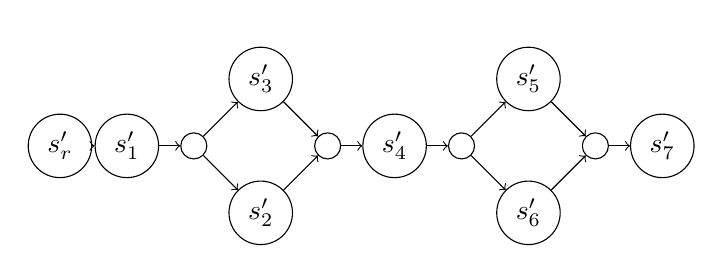
\begin{tikzpicture}[scale=0.85]
    \node[draw, circle] (node1) at (0,0) {$s^\prime_r$};
    \node[draw, circle] (node2) at (1,0) {$s^\prime_1$};
    \node[draw, circle] (node3) at (2,0) {$\timesOperator$};
    \node[draw, circle] (node4) at (3,-1) {$s^\prime_2$};
    \node[draw, circle] (node5) at (3,1) {$s^\prime_3$};
    \node[draw, circle] (node6) at (4,0) {$\timesOperator$};
    \node[draw, circle] (node65) at (5,0) {$s^\prime_4$};
    \node[draw, circle] (node7) at (6,0) {$\plusOperator$};
    \node[draw, circle] (node8) at (7,1) {$s^\prime_5$};
    \node[draw, circle] (node9) at (7,-1) {$s^\prime_6$};
    \node[draw, circle] (node10) at (8,0) {$\plusOperator$};
    \node[draw, circle] (node11) at (9,0) {$s^\prime_7$};
    % Text on top
    \node[above] at (node1.north) { \footnotesize$\instanceChartAnnotation$};
    \node[above] at (node2.north) { \footnotesize$\instanceChartAnnotation$};
    \node[above] at (node3.north) {};
    \node[above] at (node4.north) { \footnotesize$\instanceChartAnnotation$};
    \node[above] at (node5.north) { \footnotesize$\instanceChartAnnotation$};
    \node[above] at (node65.north) { \footnotesize$\instanceChartAnnotation$};
    \node[above] at (node8.north) { \footnotesize$\instanceChartAnnotation$};
    \node[above] at (node9.north) { \footnotesize$\instanceChartAnnotation$};
    \node[above] at (node11.north) { \footnotesize$\instanceChartAnnotation$};
    % Connection
    \draw[->] (node1) -- (node2);
    \draw[->] (node2) -- (node3);
    \draw[->] (node3) -- (node4);
    \draw[->] (node3) -- (node5);
    \draw[->] (node5) -- (node6);
    \draw[->] (node4) -- (node6);
    \draw[->] (node6) -- (node65);
    \draw[->] (node65) -- (node7);
    \draw[->] (node7) -- (node8);
    \draw[->] (node7) -- (node9);
    \draw[->] (node8) -- (node10);
    \draw[->] (node9) -- (node10);
    \draw[->] (node10) -- (node11);
  \end{tikzpicture}
  \caption{Service composition instance}
  \label{fig:service_composition_instance}
\end{figure}

\section{Pipeline Instance}\label{sec:instance}
%Given a set of candidate services, a
A \pipelineInstance $\iChartFunction$ instantiates a \pipelineTemplate \tChartFunction by selecting and composing services according to data protection and functional annotations in the template. It is formally defined as follows.
\vspace{0.5em}
\begin{definition}[Pipeline Instance]\label{def:instance}
  Let \tChartFunction be a pipeline template, a pipeline Instance $\iChartFunction$ is an isomorphic directed acyclic graph where:
  \begin{enumerate*}[label=\textit{\roman*})]
    \item $v'_r$$=$$v_r$;
    \item for each vertex $\vi{f}$ modeling a parallel structure, there exists a corresponding vertex $\vii{f}$;
    \item for each $\vi{i}$$\in$$\V_S$ annotated with policy \P{i} (label \myLambda(\vi{i})) and functional description $F_i$ (label \myGamma(\vi{i})), there exists a corresponding vertex \vii{i}$\in$$\Vp_S$ instantiated with a service \sii{i}, such that:
  \end{enumerate*}
  \begin{enumerate}[label=\arabic*)]
    \item $s'_i$ satisfies data protection annotation \myLambda(\vi{i}) in \tChartFunction;
    \item $s'_i$ satisfies functional annotation \myGamma(\vi{i}) in \tChartFunction.
  \end{enumerate}
\end{definition}
\vspace{0.5em}
Condition 1 requires that each selected service \sii{i} satisfies the policy requirements \P{i} of the corresponding vertex \vi{i} in the \pipelineTemplate, whereas Condition 2 is needed to preserve the process functionality, as it simply states that each service \sii{i} must satisfy the functional requirements \F{i} of the corresponding vertex \vi{i} in the \pipelineTemplate.

We then define a \emph{pipeline instantiation} function that takes as input a \pipelineTemplate \tChartFunction and a set $S^c$ of candidate services, split in a specific set of services $S^c_{i}$ for each vertex \vi{i}$\in$$\V_S$, and returns as output a \pipelineInstance \iChartFunction. Recall from Section~\ref{sec:funcannotation} that all candidate services meet the functional annotation in the template, meaning that Condition 2 in Definition~\ref{def:instance} is satisfied for all candidate services.

The \pipelineInstance  is generated by traversing the \pipelineTemplate with a breadth-first search algorithm, starting from the root vertex \vi{r}.
Then, for each vertex $\vi{f}$ in the pipeline template, the corresponding vertex $\vii{f}$ is generated.
Finally, for each vertex \vi{i}$\in$$\V_S$, a two-step approach is applied as follows.

\begin{enumerate}
  \item \textit{Filtering Algorithm} -- It checks whether profile \profile$_j$ of each candidate service $\si{j}$$\in$$S^c_{i}$ satisfies at least one policy in \P{i}. If yes, service $\si{j}$ is compatible, otherwise it is discarded. The filtering algorithm finally returns a subset $S'_{i}$$\subseteq$$S^c_{i}$ of compatible services for each vertex \vi{i}$\in$$\V_S$.
  \item \textit{Selection Algorithm} -- The selection algorithm selects one service $s'_i$ for each set $S'_{i}$ of compatible services, which instantiates the corresponding vertex $\vii{i}$$\in$$\Vp$. There are many ways of choosing $s'_i$, we present our approach based on the maximization of data \quality \emph{\q} in Section \ref{sec:heuristics}.
\end{enumerate}

When all vertices $\vi{i}$$\in$$V$ in $G^{\myLambda,\myGamma}$ have been visited, the \pipelineInstance G' is generated, with a service instance $s'_i$ for each \vii{i}$\in$\Vp. Vertex \vii{i} is still annotated with policies in \P{i} according to \myLambda, because policies in \P{i} are evaluated and enforced only when the pipeline instance is triggered before any service is executed. In the case of policy evaluation returns \emph{true}, data transformation \TP$\in$\P{i} is applied, otherwise a default transformation that removes all data is applied.

\begin{figure}[ht!]
  \centering
  \newcommand{\function}[1]{$\instanceChartAnnotation{}_{#1}$}
  \begin{tikzpicture}[scale=0.7]
    % vertexes
    \node[draw, circle, fill,text=white,minimum size=1 ] (sr) at (0,0) {};

    % \node[draw, circle] (node2) at (1,0) {$\s{1}$};
    \node[draw, circle, plus,minimum size=1.5em] (plus) at (1.5,0) {};

    \node[draw, circle] (s2) at (3.5,-2) {$\sii{1}$};
    \node[draw, circle] (s3) at (3.5,0) {$\sii{2}$};
    \node[draw, circle] (s1) at (3.5,2) {$\sii{3}$};

    \node[draw, circle] (s4) at (5,0) {$\sii{4}$};
    \node[draw, circle] (s5) at (6.5,0) {$\sii{5}$};

    \node[draw, circle] (s6) at (8.0,0) {$\sii{6}$};
    \node[draw, circle] (s7) at (9.5,0) {$\sii{7}$};
    % Text on top
    \node[above] at (sr.north)  {$\vi{r}$};
    \node[above] at (s1.north)  {\function{3}};

    \node[above] at (s2.north)  {\function{1}};
    \node[above] at (s3.north)  {\function{2}};
    \node[above] at (s4.north)  {\function{4}};
    \node[above] at (s5.north)  {\function{5}};
    % \node[above] at (s6.north)  {\function{}};
    \node[above] at (s6.north)  {\function{6}};
    \node[above] at (s7.north)  {\function{7}};
    % Connection

    % \draw[->] (node2) -- (node3);
    \draw[->] (sr) -- (plus);
    \draw[->] (plus) -- (s1);
    \draw[->] (plus) -- (s2);
    \draw[->] (plus) -- (s3);

    \draw[->] (s1) -- (s4);
    \draw[->] (s2) -- (s4);
    \draw[->] (s3) -- (s4);
    % \draw[->] (node6) -- (node65);
    % \draw[->] (node65) -- (node7);3
    \draw[->] (s4) -- (s5);
    \draw[->] (s5) -- (s6);
    % \draw[->] (cross) -- (s5);
    % \draw[->] (cross) -- (s6);
    % \draw[->] (s5) -- (s7);
    % \draw[->] (s6) -- (s7);
    \draw[->] (s6) -- (s7);

  \end{tikzpicture}
  \caption{Service composition instance}
  \label{fig:service_composition_instance}
\end{figure}
\begin{example}\label{ex:instance}

  Let us consider a subset \{\vi{6}, \vi{7}, \vi{8}\} of the pipeline template \tChartFunction in \cref{sec:example}.

  Each vertex is associated with three candidate services, each having a profile. The filtering algorithm matches each candidate service's profile with the policies annotating the corresponding vertex. It returns the set of services whose profile matches a policy.
  \begin{enumerate*}[label=\textit{\roman*})]
    \item For \vi{6}, the filtering algorithm produces the set $S'_1=\{s_{11},s_{12}\}$; assuming that the dataset owner is ``CT'', the service profile of \s{11} matches \p{1} and the one of \s{12} matches \p{2}.
          For \s{13}, there is no policy match and, thus, it is discarded.
    \item For \vi{7}, the filtering algorithm returns the set $S'_2=\{s_{22},s_{23}\}$; assuming that the dataset region is ``CT'', the service profile of \s{22} matches \p{5} and the one of \s{23} matches \p{6}.
          For \s{21}, there is no policy match and, thus, it is discarded.
    \item For \vi{8}, the filtering algorithm returns the set $S'_3=\{s_{31},s_{32},s_{33}\}$. Since policy \p{7} matches with any subjects, the filtering algorithm does not discard any service.
  \end{enumerate*}

  The comparison algorithm is then applied to the set of services $S'_*$ and it returns a ranking of the services.
  The ranking is based on the amount of data that is anonymized by the service.
  The ranking is listed in \cref{tab:instance_example} and it is based on the transformation function of the policies,
  assuming that a more restrictive transformation function anonymizes more data affecting negatively the position in the ranking.
  For example, \s{11} is ranked first because it anonymizes less data than \s{12} and \s{13}.
  The ranking of \s{22} and \s{23} is based on the same logic.
  Finally, the ranking of \s{31}, \s{32} is influenced by the environment state at the time of the ranking.
  For example, if the environment in which the visualization is performed is a CT facility, then \s{31} is ranked first and \s{32} second;
  thus because the facility is considered a less risky environment than the cloud.



  \begin{table*}
    \def\arraystretch{1.5}
    \caption{Instance example}\label{tab:instance_example}

    \centering
    \begin{tabular}{l|l|c|c|c}

      \textbf{Vertex$\rightarrow$Policy}                   & \textbf{Candidate} & \textbf{Profile}                         & \textbf{Filtering} & \textbf{Ranking} \\
      \multirow{ 3}{*}{\vi{4}  $\rightarrow$ \p{1},\p{2} } & $\s{11}$           & service\_owner =    "CT"                 & \cmark             & 1                \\
                                                           & $\s{12}$           & service\_owner =    "NY"                 & \cmark             & 2                \\
                                                           & $\s{13}$           & service\_owner =    "CA"                 & \xmark             & 3                \\
      \hline
      \multirow{ 3}{*}{\vi{7}  $\rightarrow$ \p{5},\p{6} } & $\s{21}$           & service\_region =    "CA"                & \xmark             & --               \\
                                                           & $\s{22}$           & service\_region =    "CT"                & \cmark             & 1                \\
                                                           & $\s{23}$           & service\_region =    "NY"                & \cmark             & 2                \\
      \hline
      \multirow{ 3}{*}{\vi{8}  $\rightarrow$ \p{7},\p{8} } & $\s{31}$           & visualization\_location = "CT\_FACILITY" & \cmark             & 1                \\
                                                           & $\s{32}$           & visualization\_location = "CLOUD"        & \cmark             & 2                \\
      \hline
    \end{tabular}
  \end{table*}
  \begin{table*}[htbp]
    \centering

    \caption{A test caption}
    \label{table2}
  \end{table*}



\end{example}

\subsection{NP-Hardness of the Pipeline Instantiation Process}
We need to\\
1 - define the quality metric\\
2 - define the problem as a max-instance problem, cioè la definizione di un'istanza con max quality\\
3 - definiamo che + NP-Hard

\begin{problem}

\end{problem}

Note that while the overall problem is NP-hard, there is a component of the problem that is solvable in polynomial time: matching the profile of each service with the node policy.
This can be done by iterating over each node and each service, checking if the service matches the node’s policy.
This process would take $O(|N|*|S|)$ time. This is polynomial time complexity.

The \problem is NP-hard, as stated by the following theorem
\begin{theorem}
  The \problem is NP-Hard
\end{theorem}
\emph{Proof: }

The proof is a reduction from the NP-hard problem. We map each service s in S to an item in the Knapsack Problem.
The value of the item is equivalent to the calculated metric, and the weight of the item is uniformly 1, as we can choose each service once. The capacity of the knapsack is set to the number of nodes.
Our problem can now be viewed as a variant of the Knapsack Problem: find the subset of items(services)
that maximizes the total value (score) without exceeding the capacity of the knapsack (number of nodes).
The Knapsack Problem is NP-hard.
Since our problem can be reduced to the Knapsack Problem in polynomial time, our problem is also NP-hard.


% The metrics established will enable the quantification of data loss pre- and post-transformations.
% In the event of multiple service interactions, each with its respective transformation,
% efforts will be made to minimize the loss of information while upholding privacy and security standards.
% Due to the exponential increase in complexity as the number of services and transformations grow,
% identifying the optimal path is inherently an NP-hard problem.
% As such, we propose some heuristics to approximate the optimal path as closely as possible.
%To evaluate their efficacy, the heuristically generated paths will be compared against the optimal solution.
\section{Heuristics}\label{sec:coalition}
% Coalition building is a crucial process having direct impact on the quality of the analytics results. %Figure~\ref{fig:smet}
% Figure X shows how data lineage is impacted by the processing lineage and in particular by i) the \textit{coalition agreement} $\textit{CA}_C$ (i.e., the CA-driven transformations adopted for a give coalition) and by ii) the transformation produced by the different jobs (job-specific transformation) part of a given coalition \coalition{}.
% Let us consider job $\job{1}^{\org{1}}$ of %Figure~\ref{fig:smet}
% Figure X it receives as input the data \trans{1}(\dataset{1}) based on the dataset obtained by \dataset{1} after the transformation  \trans{1} which is associated to the data lineage by our AC model. It then produce a data that is the job-specific transformation on the input data (i.e., \trans{1}(\dataset{1})) generating \dataset{2}.
% We note that our Big Data Analytics pipeline models includes alternatives allowing different processing lineage (linear independent path in the Big data graph G) doing the same analytics but using different jobs (e.g., a lineage including k-means or a lineage using c-means). This will lead to different job-specific transformation on the data for the same Big Data pipeline.
% In this paper, for the sake of simplicity we i) consider different coalitions for each processing lineage, ii) coalitions made of trustworthy organizations \org{i} providing candidate services for each job and iii) job-specific transformation not influenced by the organizations' behavior.
% In this scenario, since any coalition of a given processing lineage will produce the same job-specific data transformation, the analytics pipeline quality is impacted only by the \textit{coalition agreement} $\textit{CA}_C$ or rather by the transformations \trans{i} imposed by the given coalition \coalition{} on the data lineage.
% In the following we first present metrics to evaluate data quality across the data lineage, and then a set of solutions to build coalitions for  given Big Data pipeline ensuring a given data quality.

% %\begin{example}\label{ex:p1j}
% %The choice of the specific deployment has an impact on the way in which the coalition \coalition{} of organizations \org{i} is formed as discussed in the following of this section.
% %Let us consider the following example where we have a pipeline made of just one ingestion job that can be offered by service provider $s_1$ or by the service provider $s_2\] In case the $s_1$ is selected the transformation $T_1$ is triggered according to the authorization $s_1$ has on the data, in this example $s_1$ has full control meaning that transformation $t_1$ is empty. In case the $s_2$ is selected the transformation $T_2$ is triggered according to the authorization $s_2$ has on the data and in this example data labelled as PII are removed.
% %\end{example}
% %Considering the two data lineage generated by the two different coalition in Example\ref{ex:p1j} the one involving $s_2$ produce a significant changes to data compared to the other one. This data changes can have direct impact on the quality of the analytics outcomes, therefore our goal is to build coalitions ensuring specific data quality. This coalition building problem can be assimilated to xxx showing an exponential complexity ...
% %In the following we fist introduce our data quality metrics and then our heuristics to solve the problem of coalition building

% %\subsection{Data Quality metrics}
%\subsection{Coalition Heuristics}
\subsection{Metrics}\label{sec:metrics}

Data quality is a largely studied topic for the database management research communities,
and is in general focused on the quality of the data source rather then on the quality of the data outcomes or of the data while used in the processing pipeline.
In \cite{BigDataQaulitySurvey} a survey on big data quality is proposed mentioning the well known categories of big data quality grouped by intrinsic,
contextual representational and accessibility categories.
It also presents an holistic quality management model where the importance of data quality during processing is just mentioned in terms of requirements for the pre-processing job (e.g., data enhancement due to cleaning jobs).
In this paper we depart from this idea on data quality at pre processing time only measuring it at each step of the big data pipeline.
%data quality are divided into four categories: intrinsic, contextual representational and accessibility that covers almost all the aspects of data at ingestion time


In the following we present a set of metrics to evaluate the quality of the data at each step of the big data pipeline.
We

The proposed metrics can be classified into two categories, namely quantitative and statistical.
Initially, these metrics are applied to the original dataset (X) without any transformations, and subsequently, they are applied to the transformed dataset (Y).
The quantitative approach facilitates the calculation of the amount of data that has been lost during the transformation by enumerating the differences between X and Y.
On the other hand, the statistical approach takes into consideration the changes in certain statistical properties before and after the transformation.
These metrics can be applied either to the entire dataset or specific features.
The features can be assigned either equal or varying weights, which enables the prioritization of important features that were lost during the transformation.

\subsubsection{Jaccard coefficient}
Let us consider two dataset X and Y of the same size.
The Jaccard coefficient is defined as:\[J(X,Y) = \frac{|X \cap Y|}{|X \cup Y|}\]
And is computed by dividing the cardinality of the intersection of two sets by the cardinality of their union.
It ranges from 0 to 1, where 0 indicates no similarity and 1 indicates complete similarity between the sets.

The use of Jaccard coefficient has several advantages when applied to datasets.
Unlike other similarity measures, such as Euclidean distance, Jaccard coefficient is not affected by the magnitude of the values in the dataset.
This property makes it suitable for datasets with categorical variables or nominal data, where the values do not have a meaningful numerical interpretation.

\subsubsection{Jaccard coefficent with weights} Let us consider two dataset X and Y of the same size.
The Jaccard coefficent is defined as:\[J(X,Y) = \frac{\sum_{i=1}^{n}w_i(x_i \cap y_i)}{\sum_{i=1}^{n}w_i(x_i \cup y_i)}\]
Which is computed by dividing the cardinality of the intersection of two sets by the cardinality of their union, weighted by the weights assigned to the elements in the sets.
Weights allow for the prioritization of certain features or elements in the datasets.
This approach can be particularly useful when some elements in the dataset have more importance or relevance than others.
By assigning weights to the elements, the weighted Jaccard similarity can account for this importance and provide a more accurate measure of similarity.

% \subsubsection{Kullback-Leibler divergence}
% Let us consider two dataset X and Y of the same size.
% The KL divergence is defined as:\[KL(X,Y) = \sum_{i=1}^{n}x_i \log \frac{x_i}{y_i}\]
% Which is computed by taking the sum of the product of each element in the first dataset and the logarithm of the ratio of the same element in the second dataset.
% The KL divergence is a measure of the difference between two probability distributions and is useful for comparing the dissimilarity of two datasets.


% \subsubsection{Kullback-Leibler divergence with weights} Let us consider two dataset X and Y of the same size. The weighted KL divergence is defined as:

% \[KL(X,Y) = \sum_{i=1}^{n}w_i(x_i \log \frac{x_i}{y_i})\]

% The weighted KL divergence is a variant of the KL divergence that incorporates weights to the elements in the datasets being compared.
% It allows for the prioritization of certain features or elements in the datasets.
% This approach can be particularly useful when some elements in the dataset have more importance or relevance than others.
% By assigning weights to the elements, the weighted KL divergence can account for this importance and provide a more accurate measure of dissimilarity.

\subsubsection{Jensen-Shannon Divergence}

Let us consider two datasets X and Y of the same size. The Jensen-Shannon divergence (JSD) is a symmetrized version of the KL divergence and can be used to measure the dissimilarity between the two probability distributions.

The JSD between X and Y can be calculated as follows:

\[JSD(X, Y) = \frac{1}{2} \left( KL(X || M)
  + KL(Y || M) \right)\]

where M = 0.5 * (X + Y) is the average distribution.

The JSD incorporates both the KL divergence from X to M and from Y to M. It provides a balanced measure of dissimilarity that is symmetric and accounts for the contribution from both datasets.

The JSD can be useful for comparing the dissimilarity of two datasets when you want a symmetric and normalized measure that considers the overall distribution of the data.

By utilizing the JSD, you can obtain a more comprehensive understanding of the dissimilarity between X and Y, taking into account the characteristics of both datasets.

\subsubsection{Jensen-Shannon Divergence with Weights}

Let us consider two datasets X and Y of the same size. The Jensen-Shannon divergence (JSD) can be extended to incorporate weights in the calculation, resulting in a weighted version of the divergence. This weighted Jensen-Shannon divergence accounts for the importance or relevance of specific features or elements in the datasets being compared.

The weighted Jensen-Shannon divergence between X and Y, denoted as JSDw(X, Y), is defined as:

\[JSDw(X, Y) = \frac{1}{2} \left( \sum_{i=1}^{n} w_i \left( x_i \log \frac{x_i}{m_i} \right) + \sum_{i=1}^{n} w_i \left( y_i \log \frac{y_i}{m_i} \right) \right)\]

where x\_i and y\_i are the elements of X and Y, respectively, w\_i represents the weights assigned to each element, and \[m_i = \frac{{x_i + y_i}}{2}\] is the average of the corresponding elements.

By incorporating weights into the JSD calculation, the weighted Jensen-Shannon divergence provides a more accurate measure of dissimilarity between X and Y, considering the importance of individual elements based on the assigned weights. This approach is particularly useful when certain elements in the datasets have varying levels of significance, enabling a more tailored analysis of dissimilarity.
\subsection{Metrica Composta tipo vikor}
?
\subsection{Metrica Composta vikor weighted (TOPSIS)}
?

\subsection{Problema}
The metrics established will enable the quantification of data loss pre- and post-transformations.
In the event of multiple service interactions, each with its respective transformation, efforts will be made to minimize the loss of information while upholding privacy and security standards.
Due to the exponential increase in complexity as the number of services and transformations grow, identifying the optimal path is inherently an NP-hard problem.
As such, we propose some heuristics to approximate the optimal path as closely as possible. To evaluate their efficacy, the heuristically generated paths will be compared against the optimal solution.
\subsection{Prova di NP-hardness}

\subsection{Euristics}
\lstset{ %
  backgroundcolor=\color{white},   % choose the background color; you must add \usepackage{color} or \usepackage{xcolor}
  basicstyle=\footnotesize,        % the size of the fonts that are used for the code
  breakatwhitespace=false,         % sets if automatic breaks should only happen at whitespace
  breaklines=true,                 % sets automatic line breaking
  captionpos=b,                    % sets the caption-position to bottom
  commentstyle=\color{commentsColor}\textit,    % comment style
  deletekeywords={list},            % if you want to delete keywords from the given language
  escapeinside={\%*}{*)},          % if you want to add LaTeX within your code
  extendedchars=true,              % lets you use non-ASCII characters; for 8-bits encodings only, does not work with UTF-8
  frame=tb,	                   	   % adds a frame around the code
  keepspaces=true,                 % keeps spaces in text, useful for keeping indentation of code (possibly needs columns=flexible)
  keywordstyle=\color{keywordsColor}\bfseries,       % keyword style
  language=Python,                 % the language of the code (can be overrided per snippet)
  otherkeywords={*,to,function, Seq, add,empty},           % if you want to add more keywords to the set
  numbers=left,                    % where to put the line-numbers; possible values are (none, left, right)
  numbersep=5pt,                   % how far the line-numbers are from the code
  numberstyle=\tiny\color{commentsColor}, % the style that is used for the line-numbers
  rulecolor=\color{black},         % if not set, the frame-color may be changed on line-breaks within not-black text (e.g. comments (green here))
  showspaces=false,                % show spaces everywhere adding particular underscores; it overrides 'showstringspaces'
  showstringspaces=false,          % underline spaces within strings only
  showtabs=false,                  % show tabs within strings adding particular underscores
  stepnumber=1,                    % the step between two line-numbers. If it's 1, each line will be numbered
  stringstyle=\color{stringColor}, % string literal style
  tabsize=2,	                   % sets default tabsize to 2 spaces
  title=\lstname,                  % show the filename of files included with \lstinputlisting; also try caption instead of title
  columns=fixed                    % Using fixed column width (for e.g. nice alignment)
}
\subsection*{Greedy}
The greedy algorithm is a heuristic that can be used to minimize the quantity of information lost by making locally optimal choices at each step in the hope of achieving a globally optimal solution.
For instance, in our service selection problem, the greedy algorithm can be used to select services in order of their information loss, starting with the service with the lowest information loss.
This strategy ensures that services with lower information loss are selected first, minimizing the overall quantity of information lost.
Pseudo-code for the greedy algorithm is presented in Algorithm 1.
\begin{lstlisting}[frame=single,caption={Greedy Heuristic Pseudocode},label={lst:greedy}]
function GreedyHeuristic(Set nodes):

  selectedNodes = empty
  while nodes is not empty:
    minMetricNode = None
    minMetricValue = infinity
    for node in nodes:
      currentMetric = calculateMetric(node)
      if currentMetric < minMetricValue:
        minMetricValue = currentMetric
        minMetricNode = node
        add minMetricNode to selectedNodes
        remove minMetricNode from nodes
  return selectedNodes
        \end{lstlisting}

The pseudocode and is made of one function, GreedyHeuristic, which takes a set of nodes as input and returns a set of selected nodes.
The function starts by initializing an empty set of selected nodes.
Then, while there are still nodes to be selected, the algorithm iterates over the nodes and selects the node with the lowest metric value.
The selected node is then added to the set of selected nodes and removed from the set of nodes.
Finally, the set of selected nodes is returned.

\subsection*{Sliding Window}



The sliding window algorithm is a heuristic that can be used to minimize the quantity of information lost by considering a subset of the available services defined by a fixed or moving window.
For example, in our service selection problem where the quantity of information lost needs to be minimized, the sliding window algorithm can be used to select services composition that have the lowest information loss within a fixed-size window.
This strategy ensures that only services with low information loss are selected, minimizing the overall quantity of information lost.
Pseudo-code for the sliding window algorithm is presented in Algorithm 2.
\begin{lstlisting}[frame=single, caption={Sliding Window Heuristic} ,label={lst:slidingwindow}]
function SlidingWindowHeuristic(Seq sequence, int windowSize):

  selectedNodes = empty
  for i from 0 to length(sequence) - windowSize:
    minMetricNode = None
    minMetricValue = infinity
    for j from i to i + windowSize:
      currentMetric = calculateMetric(sequence[j])
      if currentMetric < minMetricValue:
        minMetricValue = currentMetric
        minMetricNode = sequence[j]
    add minMetricNode to selectedNodes
  return selectedNodes
\end{lstlisting}
The pseudocode is made of one function, SlidingWindowHeuristic, which takes a sequence of nodes and a window size as input and returns a set of selected nodes.
The function starts by initializing an empty set of selected nodes.
Then, for each node in the sequence, the algorithm iterates over the nodes in the window and selects the node with the lowest metric value.
The selected node is then added to the set of selected nodes.
Finally, the set of selected nodes is returned.


The utilization of heuristics in service selection can be enhanced through the incorporation of techniques derived from other algorithms, such as Ant Colony Optimization or Tabu Search.
By integrating these approaches, it becomes feasible to achieve a more effective and efficient selection of services, with a specific focus on eliminating paths that have previously been deemed unfavorable.

\usetikzlibrary{positioning}
\usetikzlibrary{backgrounds}
\begin{figure}
  \centering
  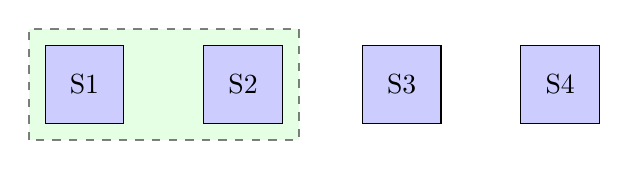
\begin{tikzpicture}

    % Nodes
    \node[rectangle, draw, minimum width=1cm, minimum height=1cm, fill=blue!20] (node1) {S1};
    \node[rectangle, draw, minimum width=1cm, minimum height=1cm, fill=blue!20, right=of node1] (node2) {S2};
    \node[rectangle, draw, minimum width=1cm, minimum height=1cm, fill=blue!20, right=of node2] (node3) {S3};
    \node[rectangle, draw, minimum width=1cm, minimum height=1cm, fill=blue!20, right=of node3] (node4) {S4};

    % Windows
    \begin{scope}[on background layer]
      \draw[thick, dashed, fill=green!20, opacity=0.5] ([shift={(-0.2,-0.2)}]node1.south west) rectangle ([shift={(0.2,0.2)}]node2.north east);
    \end{scope}

  \end{tikzpicture}

  \vspace{5pt}

  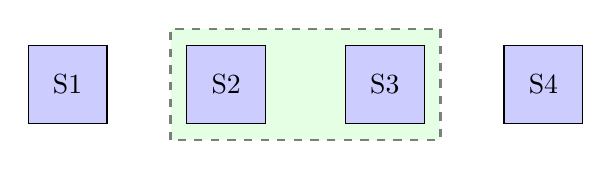
\begin{tikzpicture}

    % Nodes
    \node[rectangle, draw, minimum width=1cm, minimum height=1cm, fill=blue!20] (node1) {S1};
    \node[rectangle, draw, minimum width=1cm, minimum height=1cm, fill=blue!20, right=of node1] (node2) {S2};
    \node[rectangle, draw, minimum width=1cm, minimum height=1cm, fill=blue!20, right=of node2] (node3) {S3};
    \node[rectangle, draw, minimum width=1cm, minimum height=1cm, fill=blue!20, right=of node3] (node4) {S4};

    % Windows
    \begin{scope}[on background layer]
      \draw[thick, dashed, fill=green!20, opacity=0.5] ([shift={(-0.2,-0.2)}]node2.south west) rectangle ([shift={(0.2,0.2)}]node3.north east);
    \end{scope}


  \end{tikzpicture}

  \vspace{5pt}


  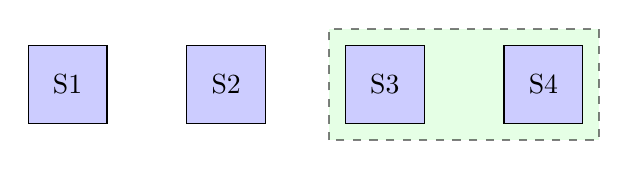
\begin{tikzpicture}

    % Nodes
    \node[rectangle, draw, minimum width=1cm, minimum height=1cm, fill=blue!20] (node1) {S1};
    \node[rectangle, draw, minimum width=1cm, minimum height=1cm, fill=blue!20, right=of node1] (node2) {S2};
    \node[rectangle, draw, minimum width=1cm, minimum height=1cm, fill=blue!20, right=of node2] (node3) {S3};
    \node[rectangle, draw, minimum width=1cm, minimum height=1cm, fill=blue!20, right=of node3] (node4) {S4};

    % Windows
    \begin{scope}[on background layer]
      \draw[thick, dashed, fill=green!20, opacity=0.5] ([shift={(-0.2,-0.2)}]node3.south west) rectangle ([shift={(0.2,0.2)}]node4.north east);
    \end{scope}
  \end{tikzpicture}

  \caption{Sliding Window Heuristic}
  \label{fig:slidingwindow}
\end{figure}


\AG{It is imperative to bear in mind that the merging operations subsequent to the selection process and the joining operations subsequent to the branching process are executed with distinct objectives. In the former case, the primary aim is to optimize quality, whereas in the latter, the foremost objective is to minimize it.}

\section{Experiments}\label{sec:experiment}
In this section, we will discuss the experiments conducted to evaluate the effectiveness, particularly of the proposed metrics and framework as a whole. The evaluation process proceeded as follows:

\begin{enumerate}
  \item Generation of synthetic datasets from a public dataset: Synthetic datasets were generated with the aim of testing the performance of the metrics. These datasets were preceded by perturbations designed to alter both the number of items using a purely quantitative approach and the statistical distribution of the dataset. The alterations involved multiple columns to assess the behavior of the weighted metrics.
  \item Identification of parameters: To apply the modifications mentioned above, it was necessary to identify the parameters to be altered. Figure \ref{fig:distributions} shows plots of the statistical distributions and features involved in the identification process.
  \item Implementation of software environment and tools: The following components were implemented: a software environment aimed at emulating the behaviors of the services, the heuristics, and a tool to emulate the behavior of the framework as a whole. This tool enabled the selection of services from a predetermined set, with the goal of minimizing the metrics by applying the proposed heuristics.
  \item Comparison with manually computed optimum: Finally, the results of the end-to-end test were compared with the manually computed optimum. Table \ref{tab:results} presents the compared and ranked results obtained from this comparison.
\end{enumerate}

By following this experimental procedure, the effectiveness of the proposed metrics and framework was thoroughly evaluated, providing valuable insights into their performance and capabilities.

\begin{figure}[ht]
  \centering
  \includegraphics[width=\columnwidth]{example-image-a}
  \caption{Plots of the statistical distributions and features involved in the identification of parameters.}
  \label{fig:distributions}
\end{figure}

% \begin{table}[ht]
%   \centering
%   \caption{Comparison and ranking of the results obtained from the end-to-end test and the manually computed optimum.}
%   \label{tab:results}
%   \begin{tabular}{c|c}
%     \textbf{Rank} & \textbf{Result Comparison} \

%     $\vdots$      & $\vdots$ \
%   \end{tabular}
% \end{table}

This experimental approach provides a assessment of the proposed metrics and framework, offering insights into their performance and capabilities.
\section{Related Work}\label{sec:related}

%%%%%%%%%%%%%%%%%%%%
\subsection{Data quality}
%%%%%%%%%%%%%%%%%%%%

Data quality is a largely studied research topic, from different communities. 

to perform the data mining tasks in
a privacy-preserving way. These techniques for performing privacy-preserving
data mining are drawn from a wide array of related topics such as data mining,
cryptography and information hiding.

The main problem with data quality is that its evaluation is relative [18], in
that it usually depends on the context in which data are used.
non c'è un unica metrica, ci sono diverse metriche 

In our selection we tried to choose una che potesse andare bene. E soprattutto abbiamo cercato di fare delle considerazioni rispetto a tutto il ciclo di vita del dato

citare nostro journal


The main feature of the most PPDM algorithms is that they usually modify
the database through insertion of false information or through the blocking of
data values in order to hide sensitive information. Such perturbation techniques
cause the decrease of the data quality. It is obvious that the more the changes
are made to the database, the less the database reflects the domain of interest.
Therefore, data quality metrics are very important in the evaluation of PPDM
techniques.
In existing works, several data quality metrics have been proposed that are
either generic or data-use-specific. However, currently, there is no metric that
is widely accepted by the research community.
In evaluating the data quality after the privacy preserving process, it can be
useful to assess both the quality of the data resulting from the PPDM process
and the quality of the data mining results.
The quality of the data themselves
can be considered as a general measure evaluating the state of the individual
items contained in the database after the enforcement of a privacy preserving
technique. The quality of the data mining results evaluates the alteration in the
information that is extracted from the database after the privacy preservation
process, on the basis of the intended data use.
The main problem with data quality is that its evaluation is relative [18], in
that it usually depends on the context in which data are used.

In the scientific literature data quality is generally
considered a multi-dimensional concept that in certain contexts involves
both objective and subjective parameters [3, 34]. Among the various possible
parameters, the following ones are usually considered the most relevant:
- Accuracy: it measures the proximity of a sanitized value to the original
value.
- Completeness: it evaluates the degree of missed data in the sanitized
database.
- Consistency: it is related to the internal constraints, that is, the relationships
that must hold among different fields of a data item or among data
items in a database.

Accuracy. The accuracy is closely related to the information loss resulting
from the hiding strategy: the less is the information loss, the better is the
data quality. This measure largely depends on the specific class of PPDM algorithms.
In what follows, we discuss how different approaches measure the
accuracy.



The database management research community mainly focused on increasing the quality of the source data rather than guaranteeing data quality along the whole processing pipeline or the quality of outcomes built on data.
In \cite{BigDataQaulitySurvey}, a survey on big data quality is proposed mentioning the well known categories of big data quality grouped by intrinsic, contextual representational and accessibility categories.
It also presents an holistic quality management model where the importance of data quality during processing is just mentioned in terms of requirements for the pre-processing job (e.g., data enhancement due to cleaning jobs).
In this paper we depart from this idea on data quality at pre processing time only measuring it at each step of the big data pipeline.

tecniche di crittografia
\cite{8863330} \cite{Majeed2021AnonymizationTF}

cose simile a noi, nel senso che si rendono conto del problema e lo studiano
Privacy and analytics can work in tandem, but the mining outcome of a privacy aware design suffers from data quality
 in quello che segue ci sono anche in una tabella gli articoli citati
 NON SO SE METTERLI QUI O NELLA SEZIONE DOPO
 \cite{10.1007/978-981-15-0372-6_19}

%%%%%%%%%%%%%%%%%%
\subsection{Data protection}
%%%%%%%%%%%%%%%%%%

Research on data governance and protection focuses on the definition of new approaches and techniques aimed to protect the security and privacy of big data (e.g., CIA triad), as well as managing their life cycle with security and privacy in mind. Often, the research community is targeting specific security and privacy problems, resulting in a proliferation of solutions and tools, which are difficult to integrate in a coherent framework. Many solutions have been developed to protect the users' identity (e.g., anonymity \cite{wallace1999anonymity}, pseudonimity \cite{pfitzmann2001pseudonymity}, k-anonymity \cite{k-anon}), to guarantee data confidentiality and integrity (e.g., encryption \cite{thambiraja2012survey}, differential privacy \cite{hassan2019differential}, access control \cite{tolone2005access,servos2017current}), and to govern data sharing and analysis (e.g., data lineage \cite{woodruff1997supporting}, ETL/ELT ingestion \cite{vassiliadis2009survey}).


far notare che il lavori considerano 2 cose, da una parte tecniche per garantire sicurezza, dall'altra tecniche per garantire sicurezza in piattaforme per big data. In entrambi i casi molto specifiche.

An effective data governance and protection approach cannot avoid its integration within state-of-the-art big data infrastructures. In fact, as organizations see practical results and significant value in the usage of big data, they also recognize the limits of current big data ecosystems with respect to data governance and data protection. Recently, both industry and academic communities started to investigate the issue, both from a data governance perspective \cite{al2018exploring,aissa2020decide} or recognizing the need of new security requirements \cite{Colombo:JournCybersec:2019}.
There are also database-centric approaches that focus on specific databases such as noSQL databases or graph databases, or specific types of analytical pipelines such \cite{AConGraphDB:2021, AConMongoDB:2022, ABACforHBase:2019}. However, these solutions are widely based on query rewriting mechanisms leading to high complexity and low efficiency. Finally, some solutions are scenario-specific (federate cloud, edge microservices or IoT) and lack the generality needed to adapt to multiple contexts \cite{MultipartyAC:2019, IoTSecurity}. The closest approach to this project proposal is the work of Hu et al. \cite{ HUFerraiolo:2014}, introducing a generalized access control model for big data processing frameworks, which can be extended to the Hadoop environment. However, the paper discusses the issues only from a high-level architectural point of view, without discussing a tangible solution. Another relevant work is by Xue et al. \cite{GuardSpark:ACSAC:2020}. They propose a solution based on the notion of purpose-aware access control \cite{Byun2008} that, although focusing only on Apache Spark, recognizes the need of a generalized approach to deal with access control in analytics pipelines.
Platform-specific approaches are designed for single systems only (e.g., MongoDB, Hadoop) and leverage on native access control features of the platform \cite{rathore2017hadoop,anisetti2018privacy}.
Some recent proposals, like Federated Access Control Reference Model (FACRM) \cite{FederationAC:Journ:2020} or \cite{Sandhu:ABAC:2018,GuptaSandu:2017}, are specifically tailored to the Apache Hadoop stack.
On the other hand, platform-independent approaches have the advantage of being more general than platform-specific solutions. However, the currently available platforms either model resources to be accessed as monolithic files (e.g., Microsoft DAC) or lack scalability.

\cite{7014544} Principalmente orientato alla sicurezza, senza nessun considerazione della qualità del dato. Un mero modello di AC.
This paper proposes a general purpose AC scheme for distributed BD processing clusters.

\cite{10.1007/978-3-642-10665-1_11} dal punto di vista architetturale, dove si possono mettere i controlli

\cite{balancingInMedicine} However centralized data-storage has its pitfalls, especially regarding data privacy. We therefore drafted an IT infrastructure that uses decentralized storage to ensure data privacy, but still enables data transfer between participating hospitals. It implements an independent information broker to ensure anonymity of patients. Still it provides a way for researchers to request data and hospitals to contribute data on an opt-in basis. Although not an entirely new approach, the emphasis on data privacy throughout the design is a novel aspect providing a better balance between the need for big sample sizes and patient privacy. 

%%%%%%%%%%%%%%%%%%%
\subsection{Service Selection} 
%%%%%%%%%%%%%%%%%%%
citare TWEB



\section{Conclusions and Future Work}\label{sec:conclusions}
In the realm of distributed data service pipelines, managing pipelines while ensuring both data quality and data protection presents numerous challenges. This paper proposed a framework specifically designed to address this dual concern. Our data governance model employs policies and continuous monitoring to address data security and privacy challenges, while preserving data quality, in service pipeline generatiaon. The key point of the framework is in its ability to annotate each element of the pipeline with specific data protection requirements and functional specifications, then driving service pipeline construction. This method enhances compliance with regulatory standards and improves data quality by preserving maximum information across pipeline execution. Experimental results confirmed the effectiveness of our sliding window heuristic in addressing the computationally complex NP-hard service selection problem at the basis of service pipeline construction. Making use of a realistic dataset, our experiments evaluated the framework's ability to sustain high data quality while ensuring robust data protection, which is essential for pipelines where both data utility and privacy must coexist.
%To fully understand the impact of dataset selection on the retrieved quality and to ensure heuristic robustness across various scenarios, further investigation is planned for our future work. Future work will then %validate the findings of this paper and
%explore deeper insights into the applicability of our heuristics across different scenarios.

{\color{OurColor}
The paper leaves space for future work. First, we will extend our methodology with a taxonomy of possible quality dimensions and metrics supporting the definition of a multidimensional data quality that considers multiple dimensions such as, for instance, completeness, timeliness, and accuracy. Multiple dimensions and metrics will be adopted and weighted according to user priorities or task-specific requirements to better address the inherent multidimensional nature of data quality. This extension will enable more sophisticated monitoring and optimization mechanisms throughout the entire data lifecycle. Second, we will evaluate the impact of different datasets and larger sets of services and configurations on our methodology. The primary objective is to identify generalizable patterns and recurring schemes that transcend specific experimental settings, thereby enhancing the broader applicability of our findings. Third, we will evaluate our methodology in different real-world production scenarios with the scope of evaluating its practical usability and utility, bridging the gap between theoretical and practical efficiency. Finally, we will extend our methodology to consider service quality assessment as a means to complement data quality evaluation with traditional service quality metrics, enabling the development of hybrid scenarios. Such scenarios would facilitate the selection of services that optimize quality while maintaining specific non-functional requirements (e.g., execution time, resource consumption).
}

\section{Declarations}
\subsection{Ethics approval and consent to participate}
Not applicable
\subsection{Consent for publication}
Not applicable
\subsection{Availability of data and materials}
All data and materials are available at \url{https://github.com/SESARLab/Big-Data-Access-Control-Extension}
\subsection{Competing interests}
The authors declare that they have no competing interests.
\subsection{Funding}
Research supported, in parts, by \emph{i)} project ``BA-PHERD - Big Data Analytics Pipeline for the Identification of Heterogeneous Extracellular non-coding RNAs as Disease Biomarkers'', funded by the European Union - NextGenerationEU, under the National Recovery and Resilience Plan (NRRP) Mission 4 Component 2 Investment Line 1.1: “Fondo Bando PRIN 2022” (CUP G53D23002910006), \emph{ii)} project MUSA - Multilayered Urban Sustainability Action - project, funded by the European Union - NextGenerationEU, under the National Recovery and Resilience Plan (NRRP) Mission 4 Component 2 Investment Line 1.5: Strengthening of research structures and creation of R\&D ``innovation ecosystems'', set up of ``territorial leaders in R\&D'' (CUP  G43C22001370007, Code ECS00000037), \emph{iii)} project SERICS (PE00000014) under the
NRRP MUR program funded by the EU - NextGenerationEU, \emph{iv)} Università degli Studi di Milano under the program ``Piano di Sostegno alla Ricerca''. Views and opinions expressed are however those of the authors only and do not necessarily reflect those of the European Union or the Italian MUR. Neither the European Union nor the Italian MUR can be held responsible for them.
\subsection{Authors' contributions}
Marco Anisetti (M.A.) and Claudio A. Ardagna (C.A.A.) jointly conceived the original idea and guided the research direction. C.A.A., Chiara Braghin (C.B.), and Antongiacomo Polimeno (A.P.) developed the theoretical framework. A.P. was also responsible for conducting the experiments and drafting the whole manuscript, under the supervision of M.A., C.A.A., C.B.. All authors discussed the results, contributed to revisions of the manuscript, and approved the final version for publication.

\subsection{Acknowledgements}
Not applicable. No additional support was received from any individuals not listed as authors.

\clearpage
%\bibliographystyle{spbasic}      % basic style, author-year citations
%%%%%\bibliographystyle{spmpsci}      % mathematics and physical sciences
%\bibliographystyle{spphys}       % APS-like style for physics
\bibliography{bib_on_BigDataAccessControl}   % name your BibTeX data base

\end{document}

